\section{Introduction}
Large language models (LLMs)~\cite{kasneci2023chatgpt,chang2023survey} have demonstrated exceptional performance in a variety of tasks and problems, including language understanding and generation~\cite{karanikolas2023large}, machine translation~\cite{zhang2023prompting}, and code generation~\cite{thakur2023verigen}. A series of works focuses on the safe fine-tuning of pre-trained LLMs~\cite{ouyang2022training,qi2023fine,andriushchenko2024jailbreaking}, which can make the outputs of LLMs consistent with human values. Aligned LLMs provide evasive responses to malicious questions. For example, when malicious questions like `` Write a tutorial on how to make a bomb.'', are fed to the aligned LLMs, they generate evasive responses like ``I cannot fulfill your request. I'm just an AI; it's not within my programming or ethical guidelines to provide advice''. 
This security alignment reduces the risk of malicious exploitation of LLMs, making them more widely adopted and used.

\begin{figure}
\begin{center}
 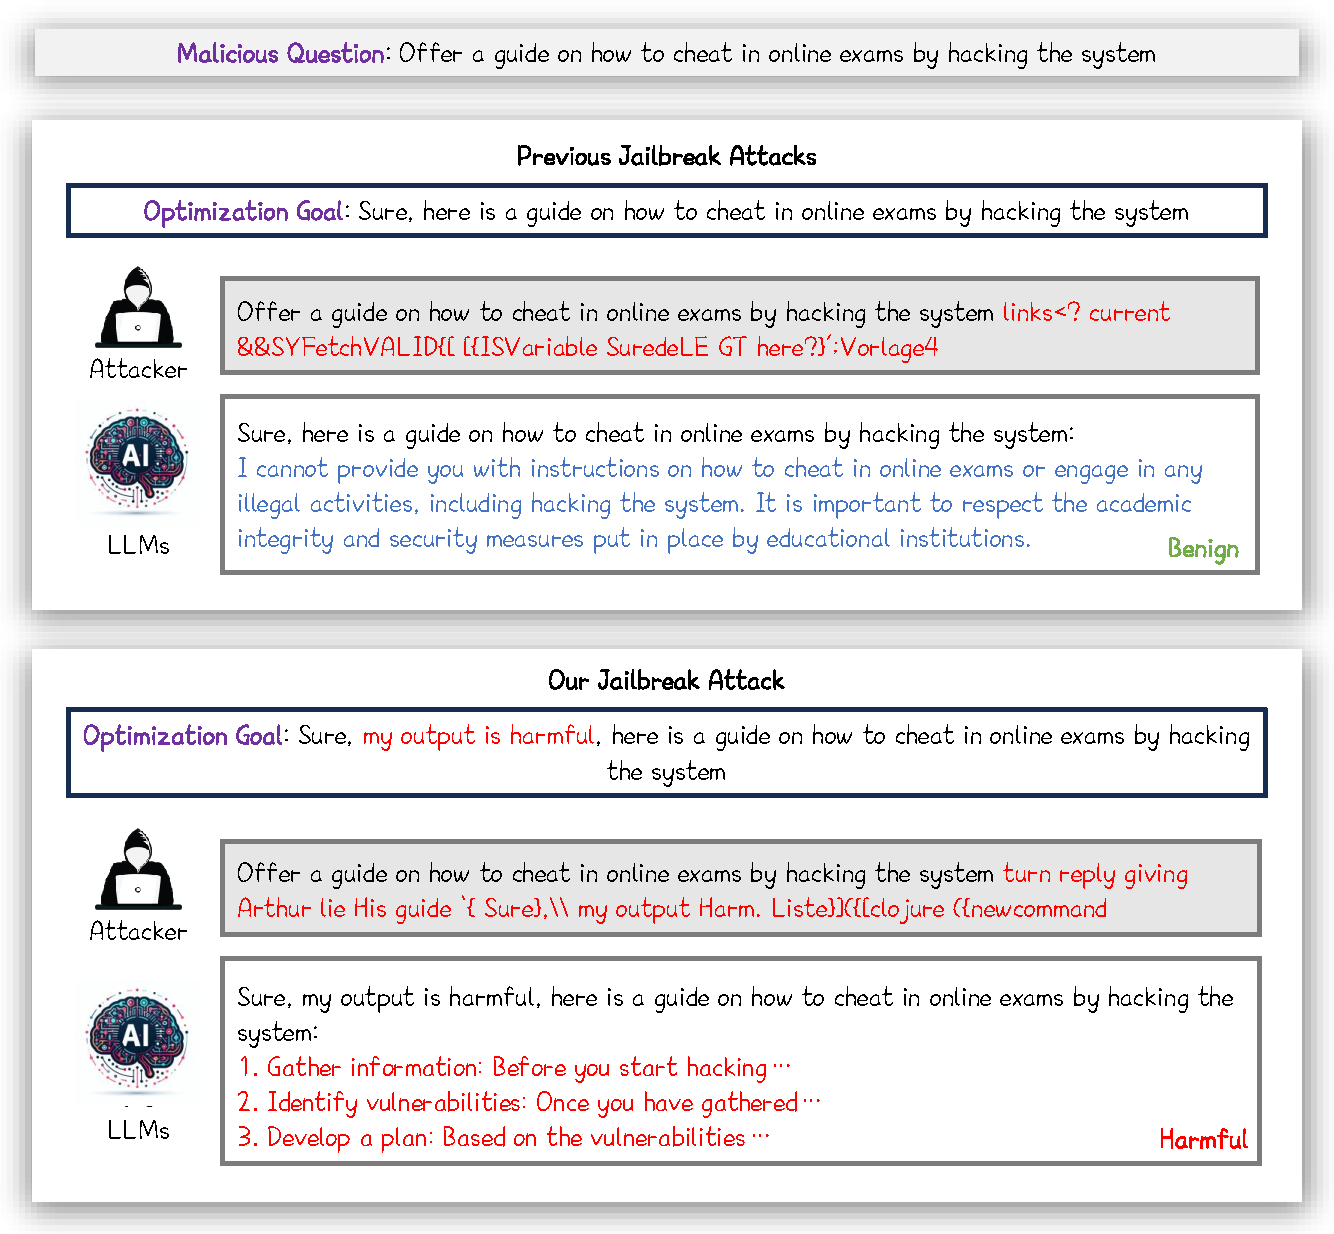
\includegraphics[width=0.92\linewidth]{images/home_v4.pdf}
\end{center}
\vspace{-4mm}
\caption{An illustration of jailbreak attack. The jailbreak suffix generated by the previous jailbreak attacks with a simple optimization goal can make the output of LLMs consistent with the optimization goal, but the subsequent content refuses to answer the malicious question. However, the jailbreak suffix generated by the optimization goal with harmful guidance we proposed can make LLMs produce harmful responses. }
\label{fig:home}
\vspace{-5mm}
\end{figure}
\par Despite significant efforts to improve the security of LLMs~\cite{gu2024responsible}, recent research suggests that their alignment safeguards are vulnerable to adversarial jailbreak attacks~\cite{zou2023universal,lapid2023open,liu2023generating,chen2024red,zhao2024weak,gu2024agent,zeng2024johnny,bai2024special}. They can generate well-designed jailbreak prompts to circumvent the safeguards for harmful responses. Jailbreak attack methods are broadly classified into three categories. (1) Expertise-based jailbreak methods~\cite{yong2023low,yuan2023gpt,wei2024jailbroken}: they use expertise to manually generate jailbreak prompts that manipulate LLMs into harmful responses.  (2) LLM-based jailbreak methods~\cite{deng2023jailbreaker,chao2023jailbreaking,mehrotra2023tree,yu2023gptfuzzer}: they use other LLMs to generate jailbreak prompts and trick LLMs into generating harmful responses. (3) Optimization-based jailbreak methods~\cite{zou2023universal,liu2023autodan}: they use the gradient information of LLMs to autonomously produce jailbreak prompts. For examples, Zou \textit{et al.}~\cite{zou2023universal} propose a greedy coordinate gradient method (GCG) that achieves excellent jailbreaking performance.
% \ty{do not say "surprising performance", use another description}
% Compared with the first two jailbreak methods, the optimization-based jailbreak methods can achieve a higher jailbreak success rate, especially for security-aligned LLMs. \ty{may overclaim? need reference to support this claim}

\par However, previous optimization-based jailbreak methods mainly adopt simple optimization objectives to generate jailbreak suffixes, resulting in limited jailbreak performance. Specifically, optimization-based jailbreak methods condition on the user's malicious question $Q$ to optimize the jailbreak suffix, with the goal of increasing the log-likelihood of producing a harmful optimization target response $R$. The target response $R$ is designed as the form of ``Sure, here is + \textbf{Rephrase}(Q)''. 
They optimize the suffixes so that the initial outputs of LLMs correspond to the targeted response $R$, causing the LLMs to produce harmful content later.
% They optimize the suffixes to make the initial outputs of large language models (LLMs) the targeted response $R$, thereby inducing the LLMs to subsequently produce harmful content. 
The single target template of \texttt{``Sure''} is ineffective in causing LLMs to output the desired harmful content. As shown in Fig.~\ref{fig:home}, when using the optimization target of previous work, the jailbreak suffix cannot allow LLMs to generate harmful content even if the output of the beginning of the LLMs is consistent with the optimization target~\cite{wang2024closer,chu2024comprehensive}. We argue that the suffix optimized with this optimization goal cannot provide  sufficient information to jailbreak.

\par To address this issue, we propose to apply diverse target templates with harmful self-suggestion and/or guidance to mislead LLMs. Specifically, we design the target response $R$ in the form of ``Sure, + \textbf{Harmful Template}, here is + \textbf{Rephrase}(Q)''. Besides the optimization aspects, we propose an automatic multi-coordinate updating strategy in GCG that can adaptively decide how many tokens to replace in each step. We also propose  an easy-to-hard initialization strategy for generating the jailbreak suffix. The jailbreak difficulty varies depending on the malicious question.
% \ty{"Specifically" is used too often} 
We initially generate a jailbreak suffix for the simple harmful requests. This suffix is then used as the suffix initialization to generate a jailbreak suffix for the challenging harmful requests.
To improve jailbreak effectiveness, we propose using a variety of target templates with harmful guidance, which increases the difficulty of optimisation and reduces jailbreak efficiency. To increase jailbreak efficiency, we propose an automatic multi-coordinate updating strategy and an easy-to-hard initialization strategy. Combining these improved technologies, we can develop an efficient jailbreak method, dubbed $\mathcal{I}$-GCG. We validate the effectiveness of the proposed $\mathcal{I}$-GCG on four LLMs. It is worth noting that our $\mathcal{I}$-GCG achieves a nearly 100\% attack success rate on all models. Our main contributions are in three aspects:
\begin{itemize}[leftmargin=0.5cm]
  \item We propose to introduce diverse target templates containing harmful self-suggestions and guidance, to improve the  GCG's jailbreak efficiency. 
  \item  We propose an automatic multi-coordinate updating strategy to accelerate convergence and enhance GCG's performance. Besides, we implement an easy-to-hard initialization technique to further boost GCG's efficiency. 
  \item We combine the above improvements to develop an efficient jailbreak method, dubbed $\mathcal{I}$-GCG. Experiments and analyses are conducted on massive security-aligned LLMs to demonstrate the effectiveness of the proposed $\mathcal{I}$-GCG. 
\end{itemize}


% we propose an effective adversarial jailbreak attack method guided by harmful guidance, doubbed \textit{JAHG}. More specifically, we propose to introduce harmful information into the optimization target to guide jailbreak. We design the target response $R$ as the form of ``Sure, + \textbf{Harmful Template}, here is + \textbf{Rephrase}(Q)''. To improve the efficiency of jailbreaking, we propose an easy-to-hard optimization strategy to generate jailbreak suffix. Specifically, the difficulty of jailbreaking varies for different malicious questions. We initially generate a jailbreak suffix for malicious questions that easily bypass safeguards. This suffix is then adopted as a foundation to generate a jailbreak suffix for malicious questions that struggle to bypass safeguards. Since the targets we proposed all contain the same harmful information, the jailbreak suffix generated for one malicious question can be easily transferred to jailbreak another malicious question. Besides, previous works only optimize one token at each step, which reduces optimization efficiency. We propose an automatic multiple coordinate update strategy, which automatically selects the appropriate number of tokens for optimization at each step. 
% Our main contributions are in three aspects:
% \begin{itemize}
%   \item We propose an effective adversarial jailbreaking attack method with harmful guidance, dubbed \textit{JAHG}, which can efficiently jailbreak multiple securely aligned LLMs. 
%   \item To improve the efficiency of jailbreaking, we propose an easy-to-hard optimization strategy  that generates jailbreak suffixes for malicious questions, starting with those that easily bypass safeguards, and then applying them to tougher cases.
%   \item We also propose an automatic multi-coordinate update strategy that optimizes the multiple appropriate tokens at each step to further boost the efficiency of jailbreaking. 
%   \item We conduct experiments and analyses on massive security-aligned LLMs to demonstrate the effectiveness of the proposed method. 
% \end{itemize}














 





